% Condition × Component heatmap (1=active=blue, 0=inactive=white)
% Rows: 12 conditions  Columns: BM25, Dense, RRF, Reranker, Refusal, Citation
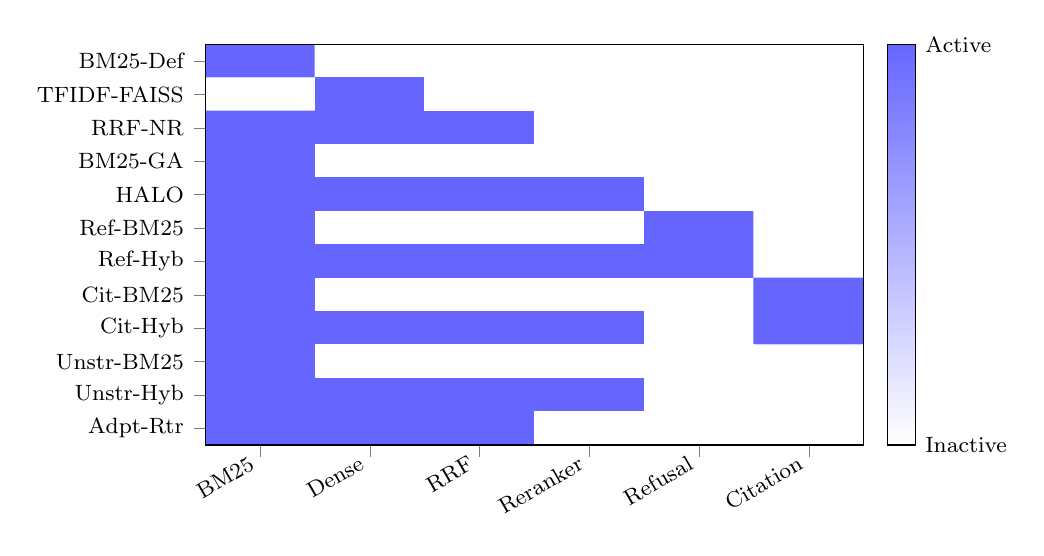
\begin{tikzpicture}
\begin{axis}[
  compat=1.18,
  width=0.82\textwidth,
  height=0.55\textwidth,
  xmin=0.5, xmax=6.5,
  ymin=0.5, ymax=12.5,
  xtick={1,2,3,4,5,6},
  xticklabels={BM25, Dense, RRF, Reranker, Refusal, Citation},
  ytick={1,2,3,4,5,6,7,8,9,10,11,12},
  yticklabels={Adpt-Rtr, Unstr-Hyb, Unstr-BM25, Cit-Hyb, Cit-BM25,
               Ref-Hyb, Ref-BM25, HALO, BM25-GA, RRF-NR, TFIDF-FAISS, BM25-Def},
  x tick label style={font=\footnotesize, rotate=30, anchor=east},
  y tick label style={font=\footnotesize},
  tick align=outside,
  tick pos=left,
  colormap={bluemap}{color(0)=(white); color(1)=(blue!60)},
  colorbar,
  colorbar style={
    ytick={0,1},
    yticklabels={Inactive, Active},
    ylabel style={font=\footnotesize},
    ticklabel style={font=\footnotesize},
    width=0.35cm,
  },
  point meta min=0, point meta max=1,
  enlargelimits=false,
  axis on top,
]

% Data: row = y coord (12=BM25-Def top, 1=Adpt-Rtr bottom)
% Columns: BM25 Dense RRF Reranker Refusal Citation
% BM25-Def    y=12: 1 0 0 0 0 0
% TFIDF-FAISS y=11: 0 1 0 0 0 0
% RRF-NR      y=10: 1 1 1 0 0 0
% BM25-GA     y=9:  1 0 0 0 0 0
% HALO        y=8:  1 1 1 1 0 0
% Ref-BM25    y=7:  1 0 0 0 1 0
% Ref-Hyb     y=6:  1 1 1 1 1 0
% Cit-BM25    y=5:  1 0 0 0 0 1
% Cit-Hyb     y=4:  1 1 1 1 0 1
% Unstr-BM25  y=3:  1 0 0 0 0 0
% Unstr-Hyb   y=2:  1 1 1 1 0 0
% Adpt-Rtr    y=1:  1 1 1 0 0 0

\addplot[matrix plot*, point meta=explicit, mesh/cols=6]
  coordinates {
    (1,12) [1]  (2,12) [0]  (3,12) [0]  (4,12) [0]  (5,12) [0]  (6,12) [0]
    (1,11) [0]  (2,11) [1]  (3,11) [0]  (4,11) [0]  (5,11) [0]  (6,11) [0]
    (1,10) [1]  (2,10) [1]  (3,10) [1]  (4,10) [0]  (5,10) [0]  (6,10) [0]
    (1,9)  [1]  (2,9)  [0]  (3,9)  [0]  (4,9)  [0]  (5,9)  [0]  (6,9)  [0]
    (1,8)  [1]  (2,8)  [1]  (3,8)  [1]  (4,8)  [1]  (5,8)  [0]  (6,8)  [0]
    (1,7)  [1]  (2,7)  [0]  (3,7)  [0]  (4,7)  [0]  (5,7)  [1]  (6,7)  [0]
    (1,6)  [1]  (2,6)  [1]  (3,6)  [1]  (4,6)  [1]  (5,6)  [1]  (6,6)  [0]
    (1,5)  [1]  (2,5)  [0]  (3,5)  [0]  (4,5)  [0]  (5,5)  [0]  (6,5)  [1]
    (1,4)  [1]  (2,4)  [1]  (3,4)  [1]  (4,4)  [1]  (5,4)  [0]  (6,4)  [1]
    (1,3)  [1]  (2,3)  [0]  (3,3)  [0]  (4,3)  [0]  (5,3)  [0]  (6,3)  [0]
    (1,2)  [1]  (2,2)  [1]  (3,2)  [1]  (4,2)  [1]  (5,2)  [0]  (6,2)  [0]
    (1,1)  [1]  (2,1)  [1]  (3,1)  [1]  (4,1)  [0]  (5,1)  [0]  (6,1)  [0]
  };

\end{axis}
\end{tikzpicture}
